%%%%%%%%%%%%%%%%%%%%%%%%%%%%%%%%%%%%%%%%%%%%%%%%%%%%%%%%%%%%%%%%%%%%%%%%%%%%%%%
%                       CARGA DE LA CLASE DE DOCUMENTO                        %
%                                                                             %
% Las opciones admisibles son:                                                %
%      12pt / 11pt            (tamaño del cuerpo de letra; no usar 10pt)      %
%                                                                             %
% catalan/spanish/english     (idioma principal del trabajo)                  %
%                                                                             % 
% french/italian/german...  (si necesitáis usar otro idioma adicional)      %
%                                                                             %
% listoffigures               (El documento incluye un Índice de figuras)     %
% listoftables                (El documento incluye un Índice de tablas)      %
% listofquadres               (El documento incluye un Índice de cuadros)     %
% listofalgorithms            (El documento incluye un Índice de algoritmos)  %
%                                                                             %
%%%%%%%%%%%%%%%%%%%%%%%%%%%%%%%%%%%%%%%%%%%%%%%%%%%%%%%%%%%%%%%%%%%%%%%%%%%%%%%

\documentclass[11pt,spanish,listoffigures,listoftables]{tfgetsinf}

%%%%%%%%%%%%%%%%%%%%%%%%%%%%%%%%%%%%%%%%%%%%%%%%%%%%%%%%%%%%%%%%%%%%%%%%%%%%%%%
%                     CODIFICACIÓN DEL ARCHIVO FUENTE                         %
%                                                                             %
%    Windows suele usar 'ansinew'                                             %
%    en Linux es posible que sea 'latin1' o 'latin9'                          %
%    Pero lo más recomendable es usar utf8 (unicode 8)                        %
%                                          (si vuestro editor lo permite)     % 
%%%%%%%%%%%%%%%%%%%%%%%%%%%%%%%%%%%%%%%%%%%%%%%%%%%%%%%%%%%%%%%%%%%%%%%%%%%%%%%

\usepackage[utf8]{inputenc} 


%%%%%%%%%%%%%%%%%%%%%%%%%%%%%%%%%%%%%%%%%%%%%%%%%%%%%%%%%%%%%%%%%%%%%%%%%%%%%%%
%                       OTROS PAQUETES Y DEFINICIONES                         %
%                                                                             %
%%%%%%%%%%%%%%%%%%%%%%%%%%%%%%%%%%%%%%%%%%%%%%%%%%%%%%%%%%%%%%%%%%%%%%%%%%%%%%%

\usepackage{glossaries}
\usepackage{textcomp}
\usepackage{booktabs}
\usepackage{float}
\usepackage{enumitem}
\usepackage{graphicx}
\usepackage{subcaption}
\usepackage{tabularx}
\usepackage{pgfplots}
\pgfplotsset{compat=1.18}

% Configuración para usar punto decimal en lugar de coma
% \usepackage{icomma}
% \decimalpoint

% Listings para código
\usepackage{listings}
\lstset{
  basicstyle=\ttfamily\small,
  frame=single,
  breaklines=true,
  postbreak=\mbox{\textcolor{gray}{$\hookrightarrow$}\space},
  columns=fullflexible,
  keepspaces=true,
  numbers=none
}

% Bibliografía
\usepackage[backend=biber,style=numeric,sorting=none]{biblatex}
\addbibresource{bibliografia.bib}

% Hyperref siempre al final
\usepackage{hyperref}
\hypersetup{
  colorlinks=true,
  linkcolor=black,
  urlcolor=cyan,
  citecolor=black
}
%%%%%%%%%%%%%%%%%%%%%%%%%%%%%%%%%%%%%%%%%%%%%%%%%%%%%%%%%%%%%%%%%%%%%%%%%%%%%%%
%                          DATOS DEL TRABAJO                                  %
%                                                                             %
% título alumno, titor y curso académico                                      %
%%%%%%%%%%%%%%%%%%%%%%%%%%%%%%%%%%%%%%%%%%%%%%%%%%%%%%%%%%%%%%%%%%%%%%%%%%%%%%%

\title{Tetris Solver \\ Jugando al Tetris con técnicas metaheurísticas}
\author{Miquel Gómez}
% \tutor{No}
% \curs{MUIARFID}

%%%%%%%%%%%%%%%%%%%%%%%%%%%%%%%%%%%%%%%%%%%%%%%%%%%%%%%%%%%%%%%%%%%%%%%%%%%%%%%
%                     PARAULES CLAU/PALABRAS CLAVE/KEY WORDS                  %
%                                                                             %
% Independentment de la llengua del treball, s'hi han d'incloure              %
% les paraules clau i el resum en els tres idiomes                            %
%%%%%%%%%%%%%%%%%%%%%%%%%%%%%%%%%%%%%%%%%%%%%%%%%%%%%%%%%%%%%%%%%%%%%%%%%%%%%%%

\keywords{
    Clasificaciò de texts.
} % Paraules clau 
{
   Clasificación de textos; Películas; Transformers; LLMs; Machine Learning
} % Palabras clave
{
    Text clasification.
} % Key words


%%%%%%%%%%%%%%%%%%%%%%%%%%%%%%%%%%%%%%%%%%%%%%%%%%%%%%%%%%%%%%%%%%%%%%%%%%%%%%%
%                                                                             %
%                              INICI DEL DOCUMENT                             %
%                                                                             %
%%%%%%%%%%%%%%%%%%%%%%%%%%%%%%%%%%%%%%%%%%%%%%%%%%%%%%%%%%%%%%%%%%%%%%%%%%%%%%%

\begin{document} 


%%%%%%%%%%%%%%%%%%%%%%%%%%%%%%%%%%%%%%%%%%%%%%%%%%%%%%%%%%%%%%%%%%%%%%%%%%%%%%%
%              RESUMENES DEL TFG EN VALENCIA, CASTELLA I ANGLES               %
%%%%%%%%%%%%%%%%%%%%%%%%%%%%%%%%%%%%%%%%%%%%%%%%%%%%%%%%%%%%%%%%%%%%%%%%%%%%%%%


\begin{abstract}[spanish]

\begin{lstlisting}[language=Python, basicstyle=\ttfamily\small, frame=single, numbers=left, breaklines=true]
def generate_prompt(df_train: pd.DataFrame, df_batch: pd.DataFrame, genres: str) -> str:
    prompt = f"""
    Classify the following movie in any of these genres. More than one genre can be assigned.
    Genres: {genres}

    ==============================================
    """

    for _, row in df_train.iterrows():
        prompt += f"Movie title: {row['movie_name']}\n"
        prompt += f"Plot: {row['description']}\n"
        prompt += f"Actual genres: {row['genre']}\n"
        prompt += "-------------------\n"

    prompt += """
    ==============================================
    Now, classify the following movies returning a structured JSON
    response with the movie names and their genres.
    """

    for _, row in df_batch.iterrows():
        prompt += f"Movie title: {row['movie_name']}\n"
        prompt += f"Plot: {row['description']}\n\n"

    return prompt
\end{lstlisting}


\end{abstract}

%%%%%%%%%%%%%%%%%%%%%%%%%%%%%%%%%%%%%%%%%%%%%%%%%%%%%%%%%%%%%%%%%%%%%%%%%%%%%%%
%                                                                             %
%                              CONTENIDO DEL TREBAJO                          %
%                                                                             %
%%%%%%%%%%%%%%%%%%%%%%%%%%%%%%%%%%%%%%%%%%%%%%%%%%%%%%%%%%%%%%%%%%%%%%%%%%%%%%%

%%%%%%%%%%%%%%%%%%%%%%%%%%%%%%%%%%%%%%%%%%%%%%%%%%%%%%%%%%%%%%%%%%%%%%%%%%%%%%%
%                                  ÍDNICE                                     %
%%%%%%%%%%%%%%%%%%%%%%%%%%%%%%%%%%%%%%%%%%%%%%%%%%%%%%%%%%%%%%%%%%%%%%%%%%%%%%%
\clearpage
\tableofcontents
% \listoffigures
% \listoftables

%%%%%%%%%%%%%%%%%%%%%%%%%%%%%%%%%%%%%%%%%%%%%%%%%%%%%%%%%%%%%%%%%%%%%%%%%%%%%%%
%                                GLOSARIO                                     %
%%%%%%%%%%%%%%%%%%%%%%%%%%%%%%%%%%%%%%%%%%%%%%%%%%%%%%%%%%%%%%%%%%%%%%%%%%%%%%%
% \glsaddall
% \printglossaries
% \printnoidxglossaries


%%%%%%%%%%%%%%%%%%%%%%%%%%%%%%%%%%%%%%%%%%%%%%%%%%%%%%%%%%%%%%%%%%%%%%%%%%%%%%%
%                                  INTRODUCCION                               %
%%%%%%%%%%%%%%%%%%%%%%%%%%%%%%%%%%%%%%%%%%%%%%%%%%%%%%%%%%%%%%%%%%%%%%%%%%%%%%%
\chapter{Introducción}

\section{Problema a resolver}
Minimización de la cobertura con restricciones 

\section{Dificultad del problema}
Escala con el número de piezas. 10 es 'fácil', 20 'medio' y 30 'difícil'. Más no por limitaciones temporales y computacionales.

%%%%%%%%%%%%%%%%%%%%%%%%%%%%%%%%%%%%%%%%%%%%%%%%%%%%%%%%%%%%%%%%%%%%%%%%%%%%%%%
%                         ANÁLISIS DEL PROBLEMA                               %
%%%%%%%%%%%%%%%%%%%%%%%%%%%%%%%%%%%%%%%%%%%%%%%%%%%%%%%%%%%%%%%%%%%%%%%%%%%%%%%
\mainmatter
\chapter{Codificación}
En este apartado se habla de como se han codificado los individuos para abordar el problema. Recordar que el objetivo es encontrar, para un set de piezas concreto, la posición y orientación óptima de cada pieza para minimizar el espacio ocupado. A eso hay que añadirle dos reglas del juego: primero que al completar una línea esta se limpia, y segundo que las piezas no pueden estar flotando al colocarse.

Con esto, se parte de la idea de 'jugar' al Tetris. La propuesta tras esta premisa no es jugar al juego de verdad, sino conseguir una codificación que permita cumplir las restricciones impuestas, consiguiendo soluciones que minimicen el espacio ocupado sin necesidad de descartar individuos inválidos. 

La forma de atacar este problema de cobertura, será definiendo una serie de movimiento posibles. Se codifica la posición final de cada pieza como una secuencia de estos. Así pues, cada genotipo será una secuencia de movimientos, de forma que si hay $x$ movimientos válidos y se dispone de $n$ piezas, la codificación de un genotipo será una secuencia $x \times n$ movimientos.

Al codificar los genotipos de esta forma, los individuos resultantes serán siempre válidos, ya que cada pieza se colocará en el tablero siguiendo las reglas del juego. Esto implica también que deberemos ser capaces de simular el juego para poder evaluar cada individuo, ya que el fenotipo de cada individuo será el estado final del tablero tras colocar todas las piezas siguiendo los movimientos indicados en el genotipo.

También, habrá movimientos que resulten en '\textit{no-op}', como intentar mover una pieza a la izquierda cuando ya está en el borde izquierdo del tablero. Más abajo vemos como se gestionan estos casos con la función objetivo.

\section{Movimientos posibles y tipos de genotipo}
Cuando decimos codificar los individuos como una secuencia de movimientos, es necesario definir cuales son estos. Si nos fijamos en el juego original, los movimientos posibles son:

\begin{itemize}
    \item Mover la pieza a la izquierda.
    \item Mover la pieza a la derecha.
    \item Rotar la pieza en el sentido de las agujas del reloj.
    \item Dejar caer la pieza.
    \item Bloquear la pieza.
    \item Intercambiar la pieza actual por la siguiente (o por una ya cambiada anteriormente)
\end{itemize}

En el juego original cuando se dejaba caer una pieza y esta toca el suelo, se bloqueaba al instante. Sin embargo, en versiones más modernas, esto no es así y aún habiendo tocado el suelo, se permite mover la pieza con unas ciertas reglas. En este caso, se hablaría hablando de un Tetris moderno como el Tetris 99 \cite{}, donde se permite que las piezas se muevan con más libertad y por tanto, se da más capacidad de representación al jugador. Es por todo esto que se ha elegido usar esta versión del juego y no la clásica. El objetivo de esta decisión es dotar a los individuos de más capacidad de representación lo que potencialmente, debería permitirnos llegar a mejores soluciones.

Ahora, si se tiene algo de experiencia en el juego, se puede ver que no en todas las situaciones, todos los movimientos son necesarios para llegar a una solución concreta. Sin ir más lejos, en casos donde el tablero está casi vacío y no hay piezas creando agujeros, siempre se podrá poner una pieza en cualquiera de las posiciones validas con una \textit{rotación} y un \textit{movimiento lateral}.

Como tampoco queremos eliminar de la experimentación la posibilidad de ver los efectos que tiene el sí hacer más movimientos una vez las piezas han tocado el suelo, se han planteado cuatro sets posibles de movimientos que podrán usar los individuos:

\begin{table}[H]
    \centering
    \begin{tabular}{ll}
        \toprule
        \textbf{Tipo} & \textbf{Secuencia de movimientos} \\
        \midrule
        Simple & \begin{tabular}[t]{@{}l@{}}
            1. Mover la pieza \\
            2. Rotar la pieza
        \end{tabular} \\
        \midrule
        Double & \begin{tabular}[t]{@{}l@{}}
            1. Mover la pieza \\
            2. Rotar la pieza \\
            3. \textit{Dejar caer la pieza} \\
            4. Mover la pieza \\
            5. Rotar la pieza
        \end{tabular} \\
        \midrule
        SwapSimple & \begin{tabular}[t]{@{}l@{}}
            1. Intercambiar la pieza actual \\
            2. Mover la pieza \\
            3. Rotar la pieza
        \end{tabular} \\
        \midrule
        SwapDouble & \begin{tabular}[t]{@{}l@{}}
            1. Intercambiar la pieza actual \\
            2. Mover la pieza \\
            3. Rotar la pieza \\
            4. \textit{Dejar caer la pieza} \\
            5. Mover la pieza \\
            6. Rotar la pieza
        \end{tabular} \\
        \bottomrule
    \end{tabular}
    \caption{Sets de movimientos posibles para los individuos.}
    \label{tab:sets_movimientos}
\end{table}
    
Donde el paso de \textit{dejar caer la pieza} NO es configurable por el individuo (es fijo) y el resto de movimientos serán un entero que indicará cuántas veces se realiza ese movimiento. Los rangos permitidos para cada tipo de movimiento se detallan en la Tabla \ref{tab:rangos_movimientos}.

\begin{table}[H]
    \centering
    \begin{tabular}{lp{8cm}}
        \toprule
        \textbf{Movimiento} & \textbf{Rango y descripción} \\
        \midrule
        Intercambiar la pieza actual & $\{0, 1\}$ \\ 
        & 0 si no se quiere intercambiar, 1 si se quiere intercambiar. \\
        \midrule
        Mover la pieza (inicial) & $\{-5, \dots, 5\}$ \\ 
        & Un entero positivo o negativo. Si es positivo, se moverá esa cantidad de veces a la derecha; si es negativo, se moverá esa cantidad de veces a la izquierda (o hasta que no se pueda mover más). \\
        \midrule
        Rotar la pieza (inicial) & $\{0, 1, 2, 3\}$ \\ 
        & Un entero entre 0 y 3, indicando cuántas veces se rotará la pieza en el sentido de las agujas del reloj. \\
        \midrule
        \textit{Dejar caer la pieza} & No configurable \\ 
        & La pieza caerá hasta que toque el suelo o otra pieza. \\
        \midrule
        Mover la pieza (final) & $\{-9, \dots, 9\}$ \\ 
        & Igual que el movimiento lateral inicial. \\
        \midrule
        Rotar la pieza (final) & $\{0, 1, 2, 3\}$ \\ 
        & Igual que la rotación inicial. \\
        \bottomrule
    \end{tabular}
    \caption{Rangos de valores permitidos para cada tipo de movimiento.}
    \label{tab:rangos_movimientos}
\end{table}

Como optimización en este punto se ha propuesto lo siguiente: dado que las piezas aparecen en cierta posición concreta, el rango de movimientos laterales que se hace al principio se ha limitado a un rango de -5 a 5. Esto es, si una pieza aparece en la columna 5 del tablero, no tendría sentido moverla más de 5 veces a izquierda o derecha (ya que se saldría del tablero).

Por último, mencionar que cuando una pieza termine de ser movida se bloqueará al momento, dejándola caer hasta tocar el suelo u otra pieza y añadiéndola al tablero.

\section{Conversión genotipo a fenotipo}
Como hemos mencionado, la idea es simular el juego a partir de los movimientos establecidos para cada pieza. De tal forma que un genotipo, representado por una secuencia de enteros (movimientos), se convierta en un fenotipo, aplicando cada jugada a la secuencia de piezas predeterminada, siendo que el estado final del tablero tras colocar todas las piezas será el fenotipo asociado.

Antes de definir un genotipo, habrá que definir un set de piezas concreto y qué movimientos se pueden realizar con cada una de ellas. A estos sets o tipos se les ha llamado \texttt{Genotype}. Con ambos datos, se podrá simular el juego con los movimientos indicados en el genotipo y el tablero final será el fenotipo asociado.

Este set de piezas será el mismo para todos los individuos, y se generará aleatoriamente al inicio de la ejecución del algoritmo. 

\section{Función objetivo}
Una vez sabemos como convertir un genotipo en fenotipo, es necesario definir una función objetivo que nos permita evaluar la calidad de cada solución. Dado que el objetivo es minimizar el espacio ocupado en el tablero, se ha definido la siguiente función objetivo:

\begin{align*}
\text{Fitness(genotipo)} = f(g) &= \text{factor juego}\times\text{puntuación juego} \\
&+ \text{factor penalización}\times\text{penalización} \\
&+ \text{factor heurísticas}\times\text{heurísticas}
\end{align*}

Desglosemos cada uno de los términos:
\begin{itemize}
    \item \textbf{Puntuación juego}: es la puntuación obtenida tras jugar la partida con el genotipo indicado. Esta puntuación se calcula como en el juego original, donde se otorgan puntos por cada línea completada, y se otorgan puntos extra por completar varias líneas a la vez (doble, triple, tetris) \cite{}. Se omiten puntos extra por combos o por dejar caer las piezas rápidamente, ya que no aportan nada a la calidad de la solución.
    
    \item \textbf{Penalización}: es una penalización que se aplica en caso de que el genotipo contenga movimientos inválidos o '\textit{no-op}' como se han definido anteriormente. La penalización será proporcional al número de movimientos inválidos realizados. Estas son calculadas durante la conversión de genotipo a fenotipo, en la simulación del juego.
    
    \item \textbf{Heurísticas}: son una serie de métricas que evalúan la calidad del tablero final tras colocar todas las piezas. En este punto es donde más se puede influir en la calidad de la solución, ya que la puntuación del juego puede ser similar para tableros muy diferentes, pero las heurísticas permitirán guiar a los algoritmos hacia mejores soluciones sin necesidad de completar muchas líneas. Además, cada heurística tendrá un peso o factor asociado, que permitirá ajustar su importancia en la función objetivo. 
\end{itemize}

\subsection{Heurísticas}
Se han definido las siguientes heurísticas para evaluar la calidad del tablero final. El origen de todas ellas es una mezcla entre heurísticas clásicas usadas en la literatura para jugar al Tetris con IA \cite{}, videos de youtube \cite{} y experiencia personal.

\begin{itemize}
    \item \textbf{Altura Agregada (Blocks)}: Suma absoluta de la cantidad de bloques que hay en el tablero. 
    \item \textbf{Altura Ponderada (Weighted Blocks)}: Similar a la anterior, pero las columnas más altas tienen un peso mayor. Esto penaliza de forma más severa la creación de picos o torres altas en el tablero.
    \item \textbf{Líneas Limpiables (Clearable Lines)}: Recompensa el número de líneas completas que se pueden eliminar con una sola pieza 'I' (la línea recta). Es una métrica directa de la puntuación que se obtendría en el juego. Su Implementación está orientada a que soluciones vecinas completen más líneas al explorar.
    \item \textbf{Rugosidad (Roughness)}: Suma de las diferencias de altura absolutas entre columnas adyacentes. Un valor alto indica un tablero no plano, lo que crea una solución peor 'compacta' y que ocupa potencialmente más espacio.
    \item \textbf{Agujeros por Columna (Column Holes)}: Número de huecos columnas con agujeros. Una agujero se define como un espacio vacío que tiene al menos un bloque por encima en la misma columna. Penaliza la creación de agujeros en las soluciones.
    \item \textbf{Agujeros Conectados (Connected Holes)}: Número de agujeros que son adyacentes a otros agujeros. Penaliza la creación de grandes bolsas de aire que son difíciles de rellenar.
    \item \textbf{Bloques sobre Agujeros (Blocks Above Holes)}: Número de bloques que se encuentran directamente encima de un agujero. Penaliza fuertemente los agujeros que están enterrados, ya que dejan grandes cavidades.
    \item \textbf{Porcentaje de Hoyos (Pit Hole Percent)}: Porcentaje de columnas que tienen un 'Hoyo'. Un hoyo se define como una columna que tiene bloques más altos en ambas columnas adyacentes. 
    \item \textbf{Hoyos más Profundo (Deepest Well)}: La profundidad de la columna más profunda de todas. Sería el mínimo de entre las alturas del bloque más alto de cada columna.
\end{itemize}

La combinación de estas heurísticas, cada una con su respectivo factor de ponderación, conforma la puntuación final de la heurística, como se muestra en la siguiente fórmula:

\begin{align*}
\text{Heurísticas} = \sum_{h \in H} w_h \times \text{score}(h)
\end{align*}

Donde $H$ es el conjunto de todas las heurísticas mencionadas, $w_h$ es el factor de ponderación para la heurística $h$, y $\text{score}(h)$ es el valor calculado para dicha heurística en el tablero final. Esta función se pretende \textbf{MAXIMIZAR}.

\subsection{Pesos de la función objetivo}
Los factores que ponderan cada uno de los términos de la función objetivo, se han establecido tras una serie de pruebas preliminares, referencias en la literatura \cite{} y 'a ojo'. Lo ideal sería poder lanzar una serie de experimentos para ajustar estos pesos, pero por limitaciones computacionales y de 'sentido' no ha sido posible.

Se dice 'sentido' porque alrededor de ajustar estos pesos, que al final no dejan de ser hiperparámetros, se podrían crear proyectos enteros. Un ejemplo sería usar técnicas metaheurísticas para ajustar estos pesos, como un algoritmo genético que optimice los pesos de las heurísticas, o incluso alguna técnica bayesiana más moderna.

Es por todo esto que al final hemos decidido fijar unos pesos 'a mano' basándonos lo mencionado anteriormente. En concreto, se han elegido los siguientes pesos:
\begin{table}[H]
    \centering
    \caption{Pesos de los componentes principales de la función objetivo.}
    \label{tab:pesos_principales}
    \begin{tabular}{lc}
        \toprule
        \textbf{Componente} & \textbf{Peso} \\
        \midrule
        Factor de Puntuación del Juego & 2.5 \\
        Factor de Penalización & -1.0 \\
        Factor General de Heurísticas & 1.0 \\
        \bottomrule
    \end{tabular}
\end{table}

A su vez, los pesos para cada una de las heurísticas individuales, que componen el término de heurísticas, se detallan en la Tabla \ref{tab:pesos_heuristicas}.

\begin{table}[H]
    \centering
    \caption{Pesos para cada heurística individual.}
    \label{tab:pesos_heuristicas}
    \begin{tabular}{lc}
        \toprule
        \textbf{Heurística} & \textbf{Peso} \\
        \midrule
        Blocks & -1.0 \\
        Weighted Blocks & -0.75 \\
        Clearable Lines & 1.0 \\
        Roughness & -1.0 \\
        Column Holes & -5.0 \\
        Connected Holes & -2.0 \\
        Blocks Above Holes & -2.0 \\
        Pit Hole Percent & -1.0 \\
        Deepest Well & -1.0 \\
        \bottomrule
    \end{tabular}
\end{table}

Como vemos, gran parte de estos factores son negativos. El problema a solucionar es minimización del espacio ocupado, pero la función objetivo está planteada como maximización. La idea tras todo esto es que \textbf{estas heurísticas codifiquen el concepto de 'minimización del espacio'} y guíen la búsqueda de soluciones. Por lo tanto, se penaliza todo aquello que aleje al tablero de este ideal y se recompensa lo que lo acerque.

\subsection{Notas}
Comentar ciertos aspectos importantes a modo de resumen sobre la función objetivo:
\begin{itemize}
    \item Como se ha mencionado, el problema consiste en la minimización del espacio ocupado. La función objetivo \textbf{codifica este concepto a través de las heurísticas}, que penalizan tableros con mucho espacio vacío, agujeros, rugosidad, etc.
    \item La puntuación del juego se incluye para incentivar la eliminación de líneas, que es un objetivo secundario pero relevante en el Tetris y puede ayudar a la búsqueda de soluciones óptimas, ya que al limpiar piezas, se libera espacio en el tablero.
    \item La penalización por movimientos inválidos, se incluye para evitar penalizar individuos con movimientos innecesarios. Ya que simulamos el juego, NO tenemos individuos inválidos, pero siempre preferimos individuos que usen todos sus movimientos a aquellos que no se intentan mover innecesariamente.
\end{itemize}

    
%%%%%%%%%%%%%%%%%%%%%%%%%%%%%%%%%%%%%%%%%%%%%%%%%%%%%%%%%%%%%%%%%%%%%%%%%%%%%%%
%                           TÉCNOLOGÍAS PLANTEADAS                            %
%%%%%%%%%%%%%%%%%%%%%%%%%%%%%%%%%%%%%%%%%%%%%%%%%%%%%%%%%%%%%%%%%%%%%%%%%%%%%%%
\chapter{Implementación}
En este capítulo se describen las tecnologías y herramientas usadas para implementar las soluciones propuestas en este trabajo. Se habla del lenguaje de programación, librerías y frameworks usados, así como de la arquitectura general del sistema.

%%%%%%%%%%%%%%%%%%%%%%%%%%%%%%%%%%%%%%%%%%%%%%%%%%%%%%%%%%%%%%%%%%%%%%%%
\section{Tecnología de Implementación}
El desarrollo del proyecto se ha realizado mayoritariamente en C\#. Para lo que sería la parte visual se ha utilizado el framework Unity \cite{}, que permite crear aplicaciones gráficas de forma sencilla y rápida. También se ha usado Python para la visualización de resultados y generación de gráficos.

La implementación del juego se ha hecho mediante C\# y Unity de forma que se han podido representar las soluciones de forma visual y dinámica. Unity permite crear escenas 2D y 3D de forma sencilla, y cuenta con una gran comunidad y documentación, por lo que para simular un juego como el Tetris, es una opción muy adecuada.

Respecto a la implementación de los algoritmos metaheurísticos, se ha optado por usar C\# para mantener la coherencia con el resto del proyecto. C\# es un lenguaje potente y versátil, que permite implementar algoritmos complejos de forma eficiente y sin tener tantas complicaciones técnicas como C or C++.

Los resultados de los experimentos se han almacenado en logs, de forma que se puedan analizar posteriormente.

Por último, para la visualización de estos resultados, su análisis y generación de gráficos, se ha usado Python con librerías como Matplotlib \cite{} y Plotly \cite{}. Estas librerías permiten crear gráficos de forma sencilla y personalizable, lo que facilita la presentación de los resultados obtenidos en los experimentos.

La Implementación de todo el código se puede encontrar en el repositorio de GitHub \cite{}.

\section{Implementación del Tetris}
Como ya se ha mencionado, la versión del Tetris utilizada es una versión moderna. Para tener control absoluto del juego y su simulación, se ha implementado el juego desde cero usando la guía oficial para el desarrollo de juegos Tetris \cite{}.

Para poder hacer la simulación del juego, se ha abstraído todo mediante clases y objetos que representan las piezas, el tablero y las reglas del juego. De esta forma, se puede simular el juego de forma independiente de la parte visual y la parte lógica de los algoritmo. 

La Implementación se ha realizado de la forma más optima posible, eliminando operaciones innecesarias y optimizando el código para que la simulación sea lo más rápida posible. Se planeaba paralelizar los experimentos, pero por limitaciones de Unity el resultado era más lento que la versión secuencial, por lo que se ha optado por dejar el paralelismo para futuros trabajos.

De igual forma, el cálculo de la función objetivo y las heurísticas se ha optimizado al máximo, evitando cálculos redundantes y almacenando resultados intermedios cuando es posible. Por ejemplo, en el algoritmo genético se evitaba re-calcular la función objetivo para individuos que no hayan sido reemplazados entre generaciones, más detalles en el capítulo de su Implementación.

%%%%%%%%%%%%%%%%%%%%%%%%%%%%%%%%%%%%%%%%%%%%%%%%%%%%%%%%%%%%%%%%%%%%%%%%%%%%%%%
%                           ALGORITMOS                                   %
%%%%%%%%%%%%%%%%%%%%%%%%%%%%%%%%%%%%%%%%%%%%%%%%%%%%%%%%%%%%%%%%%%%%%%%%%%%%%%%
\chapter{Algoritmos}
En esta sección, se presentan los algoritmos implementados y las decisiones de diseño tomadas durante su desarrollo. La sección se centra en las técnicas y operadores utilizados de cada algoritmo.

El proceso de desarrollo incluyó una exploración manual inicial de parámetros y técnicas no documentada, motivada por las limitaciones temporales del curso. Esta fase preliminar ha servido para acotar la experimentación exhaustiva que se ha hecho más tarde, lo que ha permitido identificar los enfoques que prometen los mejores resultados.

Las decisiones finales sobre los algoritmos y el razonamiento de su elección se detallan aquí, mientras que los parámetros específicos que se usaron en la experimentación se explican en la sección de Experimentación. No se pretende omitir todo lo experimentado, sino que se hablará del porqué de las decisiones junto con las alternativas consideradas.

Además, ya que esta memoria tiene como principal objetivo el ser evaluada por el profesor responsable de la asignatura, no se entrará en detalles básicos sobre el funcionamiento de los algoritmos, sino que se explicarán la forma en la que ha implementado cada parte de ellos.

\section{Algoritmo genético}
El algoritmo genético (Genetic Algorith, GA) \cite{} se ha implementado siguiendo los principios básicos de esta técnica de optimización. Siguiendo lo mencionado anteriormente, se habla de como se llevan a cabo los pasos del algoritmo, en concreto: de la Población inicial, el Cruce, la Mutación, la Selección y el Reemplazo.

\subsection{Población inicial}
En esta sección se habla de los pasos a seguir para generar individuos nuevos. En las solución final propuesta solo se generan nuevos individuos al inicio. Sin embargo, se ha experimentado incluyendo nuevos individuos en cada generación, pero los resultados no han sido concluyentes por falta de pruebas más exhaustivas. Es por ello que se ha optado por una población inicial fija.

El número de individuos generados es un hiperámetro y se mantendrá constante durante toda la ejecución del algoritmo. A su vez, hay que definir el tipo de individuo a generar (el set de movimientos) junto con el número de piezas con las que se hará la optimización.

Una vez definidos estos parámetros, se generan los N individuos de forma independiente rellenando sus sets de movimientos. Vamos a indicar como se haría para el tipo de individuo \texttt{SwapDouble}, el resto de tipos son iguales pero con menos movimientos.

\begin{enumerate}
    \item Para cada individuo $i$ desde $1$ hasta $N$:
    \begin{enumerate}
        \item Crear un nuevo $individuo_i$ vacío
        \item Para cada pieza $j$ desde $1$ hasta $P$:
        \begin{enumerate}
            \item Generar $swap \gets$ entero aleatorio en $\{0, 1\}$
            \item Generar $movLateralInicial \gets$ entero aleatorio en $\{-5, \dots, 5\}$
            \item Generar $rotacionInicial \gets$ entero aleatorio en $\{0, 1, 2, 3\}$
            \item Generar $movLateralFinal \gets$ entero aleatorio en $\{-9, \dots, 9\}$
            \item Generar $rotacionFinal \gets$ entero aleatorio en $\{0, 1, 2, 3\}$
            \item Añadir todos estos movimientos a $individuo_i$ para la pieza $j$
        \end{enumerate}
    \end{enumerate}
    \item Devolver la población con los $N$ individuos generados
\end{enumerate}

Recordamos que cada movimiento está acotado a un rango concreto para evitar la mayor cantidad de movimiento inválidos posibles. Aún así, como se ha mencionado en la sección de la función objetivo, se penalizan los \textit{no-op}s para evitar que los individuos generen movimientos innecesarios.

\subsection{Selección}
Para la selección se ha optado por probar tanto el método elitista como el método de tarta. 

Para el método elitista se probaron varios tamaños de élite, pero a la larga no se conseguían buenas soluciones, quedando el algoritmo rápidamente estancado en óptimos locales. 

Por otro lado, el método de tarta parecía tener llegar a buenos resultado, por lo que se ha optado por usar este método en la solución final. En este método, se seleccionan dos padres para el cruce de forma proporcional a su fitness. Es decir, cuanto mejor sea el fitness de un individuo, más probabilidad tendrá de ser seleccionado como padre.

A todos los individuos se les asigna una probabilidad usando la función Softmax \cite{}. Esta función transforma los valores de fitness en probabilidades entre 0 y 1, de forma que la suma de todas las probabilidades sea 1. 

Al inicio se ha optado por usar la Softmax 'pura', pero se ha visto que los individuos con mejor fitness acaparaban casi toda la probabilidad de ser seleccionados, por lo que se ha optado por escalar con la versión 'temperatura' de la Softmax. Esta versión introduce un parámetro de temperatura $T$ que controla la 'suavidad' de la distribución de probabilidades. A mayor $T$, más uniforme será la distribución (más exploración), y a menor $T$, más se acentuará la diferencia entre los individuos, seleccionando solo los mejores (más explotación).

Haciendo varias pruebas se ha optado por una escala de decremento de la temperatura con decremento logarítmico con la formula:
\begin{align*}
    temp = \max(0.1\quad, \quad\frac{InitialTemp}{\log(generationI + 2)})
\end{align*}

Se han probado distintas temperaturas iniciales, pero al final se ha optado por una temperatura MUY alta que favorece la exploración de $InitialTemp = 100$. 

\begin{figure}[H]
    \centering
    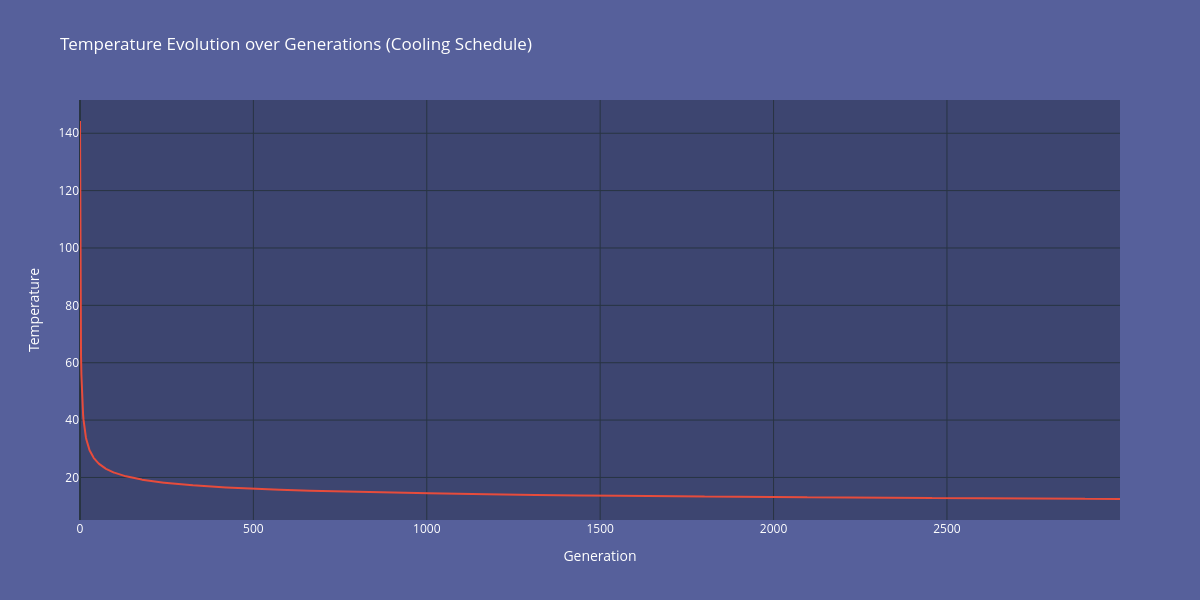
\includegraphics[width=0.7\textwidth]{images/GA_temp_evolution.png}
    \caption{Evolución de la temperatura a lo largo de las generaciones.}
    \label{fig:temp_evolution}
\end{figure}

Como vemos en la gráfica, siempre usamos valores muy elevados de temperatura. A lo largo de la memoria se hará más incapié en este punto, pero la EXPLORACIÓN es lo que más ha beneficiado a la generación de buenas soluciones. En sa línea se seleccionan más parámetros en los siguientes puntos.

\subsection{Cruce}
El cruce parte de poder usar la función de selección para elegir dos padres. Con ellos, se generan dos hijos usando el operador que junta la mitad de las piezas de cada padre para generar un hijo. El proceso es el siguiente:

\begin{enumerate}
    \item Seleccionar dos padres $padre_1$ y $padre_2$ usando la función de selección.
    \item Crear hijo $hijo_1$ usando la primera mitad de 'piezas' del $padre_1$ y la segunda mitad de 'piezas' de $padre_2$.
    \item Crear hijo $hijo_2$ usando la primera mitad e 'piezas' del $padre_2$ y la segunda mitad de 'piezas' del $padre_1$.
    \item Mutar con probabilidad $p_{mutacion}$ hijo $hijo_1$ (ver sección de mutación).
    \item Mutar con probabilidad $p_{mutacion}$ hijo $hijo_2$ (ver sección de mutación).
    \item Devolver $hijo_1$ y $hijo_2$.
\end{enumerate}

Cuando se dice 'piezas', se hace referencia a todos los movimientos asociados a cada pieza concreta. Por ejemplo, en el tipo de individuo \texttt{Simple}, cada pieza tiene dos movimientos asociados (movimiento lateral inicial, rotación inicial). Por lo tanto, si se está optimizando con diez piezas al hacer el cruce, se copian todos los movimientos asociados a las piezas $\{1\dots5\}$ del $padre_1$ y las $\{6\dots10\}$ del padre $padre_2$ para generar $hijo_1$, mientras que se copian los movimientos de las piezas $\{1\dots5\}$ del $padre_2$ y las $\{6\dots10\}$ del $padre_1$ para generar $hijo_2$.

Ya que ambos padres se codifican como una secuencia de enteros, se podría explicar como
\begin{align*}
padre_1 &= [m_{1,1}, m_{1,2},  m_{2,1}, m_{2,2} \dots, m_{10,1}, m_{10,2}] \\
padre_2 &= [m'_{1,1}, m'_{1,2},  m'_{2,1}, m'_{2,2} \dots, m'_{10,1}, m'_{10,2}] \\
hijo_1 &= [m_{1,1}, m_{1,2},  m_{2,1}, m_{2,2} \dots, m_{5,1}, m_{5,2}, m'_{6,1}, m'_{6,2} \dots, m'_{10,1}, m'_{10,2}] \\
hijo_2 &= [m'_{1,1}, m'_{1,2},  m'_{2,1}, m'_{2,2} \dots, m'_{5,1}, m'_{5,2}, m_{6,1}, m_{6,2} \dots, m_{10,1}, m_{10,2}]
\end{align*}

Por la naturaleza del problema, es apropiado hacer un cruce a nivel de \textbf{piezas continuas}, y no elegir piezas alternadamente de un padre y de otro. La razón tras esto es la dependencia que hay entre una pieza y todas aquellas colocadas a continuación. Si se mezclan piezas de ambos padres de forma alternada, se puede romper la coherencia entre las piezas y generar soluciones peores con mayor probabilidad. Esto se ha descubierto tras probar ambos métodos, y ver que el cruce por piezas continuas generaba mejores soluciones de forma consistente.

También se ha probado creando solo un hijo en lugar de dos y / o NO usando ningún padre (es decir solo mutar). A la larga ninguna otra combinación ha dado mejores resultados que la propuesta, por lo que se ha optado por esta.

\subsection{Mutación}
La mutación se aplica al individuo resultante del cruce de dos padres con una probabilidad determinada. De nuevo, este será un hiperámetro a definir en la experimentación y cada hijo resultante de un cruce se selecciona para ser mutado de forma independiente con probabilidad $p_{mutacion}$.

Una vez un individuo ha sido elegido para ser mutado, se hace lo siguiente:
\begin{enumerate}
    \item Seleccionar una pieza al azar del individuo.
    \item Seleccionar un movimiento al azar dentro de esa pieza.
    \item Mutar el movimiento seleccionado generando un nuevo 'valor aleatorio total' dentro del rango permitido para ese movimiento.
\end{enumerate}

Como ya se ha comentado anteriormente, para cada tipo de movimiento hay un rango permitido \ref{appendix:movimientos}. Se han planteado dos formas de elegir el nuevo valor del movimiento:
\begin{itemize}
    \item \textbf{Mutación aleatoria total}: generar un nuevo valor aleatorio dentro del rango permitido para ese movimiento.
    \item \textbf{Mutación cercana}: generar un nuevo valor cercano al valor actual del movimiento.
\end{itemize}

Cuando se dice 'mutaciones cercanas', se hace referencia al hecho de NO variar el valor actuar en más de uno y solo elegir 'vecinos inmediatos'. Por ejemplo, si el movimiento es un desplazamiento lateral de 3, solo se mutaría a 2 o 4 en la versión cercana, pero en la aleatoria total se generaría un nuevo valor aleatorio entre -5 y 5 (en este caso).

La razón de aplicar la estrategia de mutación aleatoria total, es aumentar la diversidad de la población y poder escapar de óptimos locales con mayor probabilidad. Se han probado ambos formatos y la generación de soluciones buenas se veía muy ralentizada al aplicar mutaciones cercanas. Es por ello que se ha optado por usar mutaciones aleatorias totales en la solución final.

\subsection{Reemplazo}
El reemplazo como ya se sabe consiste en decidir qué de la generación actual pasan a la siguiente y cuales son reemplazados. 

Sin muchas sorpresas, se ha optado por un reemplazo generaciónal parcial, donde la mitad peor de individuos es totalmente reemplazada por aquellos creados mediante el cruce y la mutación.

Ya que por cada cruce se generan dos hijos, se realizan $N/4$ cruces para generar $N/2$ nuevos individuos que reemplazan a la mitad peor de la población actual. 

Cabe destacar que además, a la hora de evaluar las fitness de la nueva generación y ordenar los individuos, nos ahorramos la mitad de los cálculos al haber mantenido la mitad de la generación anterior. Esto es, solo se evalúan los $N/2$ nuevos individuos y se combinan con los $N/2$ individuos de la generación anterior, cuyos fitness ya se conocen.


\section{Enfriamiento simulado}
De forma similar a como se ha hecho en el apartado anterior, para el Enfriamiento simulado (Simulated Annealing, SA) \cite{} se ha implementado siguiendo los principios básicos de esta técnica de optimización. Siguiendo lo mencionado en la introducción a este apartado, se habla de como se llevan a cabo los pasos del algoritmo, en concreto: la definición de Vecindario, la lista Tabu, la Paciencia y el Enfriamiento de la temperatura.

Primero que todo mencionar que, a diferencia del algoritmo genético, el Enfriamiento simulado parte de un único individuo inicial y va explorando soluciones vecinas a este individuo. Por lo tanto, no hay una población de individuos, sino un único individuo que se va actualizando a lo largo de la ejecución del algoritmo.

Este individuo es generado de forma aleatoria al inicio, de forma similar a como se ha hecho en la sección de Población inicial del algoritmo genético. Se plantea más abajo el usar como individuo inicial el mejor individuo encontrado por el algoritmo genético, pero por limitaciones de tiempo no se ha podido implementar.

Recordar también que el algoritmo de Enfriamiento simulado tiene un parámetro de temperatura que controla la probabilidad de aceptar soluciones peores a la actual. Si una mejor solución aparece SIEMPRE la elegimos, pero si no, se acepta con una probabilidad que depende de la temperatura, de forma que se pueda escapar de óptimos locales. Ya que estamos maximizando, la probabilidad de aceptar en estos casos se calcula como:

$$
P(aceptar) = \min(1, \quad e^{\frac{\Delta fitness}{temp}})
$$

Donde $\Delta fitness$ es la diferencia de fitness entre la solución actual y la nueva solución vecina, y $temp$ es la temperatura actual del sistema.

\subsection{Vecindario}
Una vez tenemos este individuo inicial, es necesario definir cómo se generan soluciones vecinas a partir de él.

Dada la naturaleza del problema y la codificación elegida, no hay otra forma de definir el vecindario que no sean aquellos individuos cuyos valores en el genotipo difieran en un único movimiento. Es decir, se generan soluciones vecinas mutando un único movimiento del individuo actual.

La primera implementación de este vecindario se hizo usando la mutación cercana, es decir, generando un nuevo valor cercano al valor actual del movimiento. Sin embargo, tras varias pruebas se vio que este método no generaba soluciones vecinas suficientemente diversas, por lo que se optó por usar la mutación aleatoria total, generando un nuevo valor aleatorio dentro del rango permitido para ese movimiento. \textit{Se observa lo mismo que antes, la exploración limitada de mutaciones cercanas no permite escapar de óptimos locales.}

Con algo más de experimentación se vió que este método generaba buenas soluciones, pero parecía saltarse algunas posibles intermedias o se quedaba estancado sin saltar de individuo. Por ello, se ha terminado optando por generar una lista de todos los movimientos posibles para cada pieza (según el tipo de individuo) e iterar sobre todas ellas para generar soluciones vecinas de forma ordenada. Cuando todas las soluciones de una pieza han sido exploradas, se pasa a la siguiente pieza y se repite el proceso hasta haber explorado todas las piezas.

La forma en la que se generan esta lista es simple y compleja a la vez, ya que se hace optimizando el espacio y no generando de verdad todas las combinaciones. Partimos de saber todos los valores posibles para cada movimiento (ver Apéndice \ref{appendix:movimientos}), así pues es posible indexar en una lista los valores que puede tener cada movimiento. Por ejemplo, si estamos en \texttt{SwapSimple}, los posibles valores son 

$$
[0, 1, \quad -5, -4, -3, -2, -1, 0, 1, 2, 3, 4, 5, \quad 0, 1, 2, 3]
$$

Donde los primeros dos valores corresponden al intercambio de pieza, los siguientes once al movimiento lateral inicial, y los últimos cuatro a la rotación inicial.

Ya que estos $M$ movimientos son fijos, y se tienen $N$ piezas, se puede iterar de $0$ a $N\times M - 1$ con un índice $idx$ y calcular a qué pieza y movimiento corresponde dicho valor, intercambiarlo generando un nuevo individuo y evaluarlo. El cálculo es el siguiente:

\begin{lstlisting}[language={[Sharp]C}, basicstyle=\ttfamily\small, frame=single, numbers=left, breaklines=true]
// Create a neighbor by mutating the current best genotype
int pieceIndex = idx % nPieces;
int moveTypeIndex = (idx / nPieces) % allMovements.Length;
int valueIndex = idx / (nPieces * allMovements.Length);

// Ensure valueIndex is within bounds
valueIndex = valueIndex % allMovements[moveTypeIndex].Length;
\end{lstlisting}

Con esto, cada vez que se itera sobre $idx$, se obtiene la pieza y el movimiento a modificar, junto con el nuevo valor a asignar. De esta forma, se exploran todas las soluciones vecinas de forma ordenada. Si al terminar de explorar todas las soluciones NO se ha encontrado una mejor solución, se reinicia el índice $idx$ a $0$ y se vuelve a empezar (con una temperatura menor, ver sección de Enfriamiento de la temperatura).

También, mencionar que para añadir estocasticidad a la exploración, no se empieza por $idx = 0$, sino que se genera un valor aleatorio entre $0$ y $N \times M - 1$ para empezar la exploración desde ahí. De esta forma, se evita explorar siempre las mismas soluciones en el mismo orden, lo que podría llevar a estancamientos.

\subsection{Lista Tabu}
Debido a la naturaleza del vecindario y la forma en la que se exploran las soluciones vecinas, es posible que el algoritmo vuelva a explorar soluciones ya visitadas. Además, por las dependencias que se crean entre las primeras y últimas piezas, podemos intuir que el espacio se soluciones está lleno de valles gigantes en los que se puede ver estancado el algoritmo. 

Para evitar esto, se ha implementado una lista Tabu que almacena los últimos $K$ individuos visitados. De esa forma, cuando se vaya a explorar una nueva solución, se comprobará si ya ha sido visitada anteriormente. En tal caso, se descartará y se generará una nueva solución en su lugar.

El tamaño de la lista Tabu $K$ es un hiperámetro a definir en la experimentación. Se han probado distintos valores para esta lista, en la fase de experimentación se definen cuales han sido los candidatos en los experimentos. 

\subsection{Paciencia y Enfriamiento de la temperatura}
La idea principal del enfriamiento simulado, es definir un parámetro de exploración / explotación que vaya variando a lo largo de la ejecución. El valor de este parámetro marca la probabilidad de aceptar soluciones peores a la actual, de forma que se pueda escapar de óptimos locales y no quedarse atrapado en ellos.

Después de probar distintas formas de variar valor, se ha optado por usar una temperatura inicial alta que vaya decreciendo linealmente a lo largo de la ejecución con un factor de enfriamiento (también hiperparámetros). En cada iteración, el valor de la temperatura se reduce con la fórmula:

$$
temp_i = \max(0.1\quad, \quad temp_{i-1}\times (1 - coolingFactor))
$$

Ahora, no podemos siempre decrementar este valor, hay que ser conscientes de si el algoritmo se está quedando estancado o no. La forma de medir este estancamiento se controla mediante una 'paciencia'. 

Si durante $T_paciencia$ iteraciones no se encuentra una mejor solución a la actual (que no mejor solución global), se puede considerar que el algoritmo está estancado y en cada iteración se aumenta la temperatura con la siguiente fórmula:

$$
temp_i = \max(0.1\quad, \quad temp_{i-1} \times (1 + coolingFactor))
$$

De esta forma, si el algoritmo se queda estancado, se aumenta la temperatura para favorecer la exploración y poder escapar de óptimos locales. Si se encuentra una mejor solución, se resetea el contador de paciencia y se vuelve a decrementar la temperatura en cada iteración.

\subsection{Temperatura inicial}
Tras diversas pruebas y ver el comportamiento del algoritmo, se ha visto que con temperaturas medianas / elevadas el algoritmo parece elegir y saltar a soluciones peores con demasiada frecuencia y no consigue 'nada' hasta que el valor no baja de 1. 

Es así como se ha optado por elegir $temp_{initial} = 2$, de forma que el algoritmo tenga iteraciones suficientes para explorar, pero no haga una gran cantidad de forma innecesaria sin encontrar un camino por el que poder avanzar.

%%%%%%%%%%%%%%%%%%%%%%%%%%%%%%%%%%%%%%%%%%%%%%%%%%%%%%%%%%%%%%%%%%%%%%%%%%%%%%%
%                           EXPERIMENTACIÓN                                   %
%%%%%%%%%%%%%%%%%%%%%%%%%%%%%%%%%%%%%%%%%%%%%%%%%%%%%%%%%%%%%%%%%%%%%%%%%%%%%%%
\chapter{Experimentación}
En este capítulo se describen los experimentos realizados para evaluar el rendimiento de los algoritmos implementados. Se detallan los parámetros probados de cada algoritmo, en que rango se han explorado y las decisiones tomadas para elegir los valores finales usados en la sección de Resultados.

\section{Algoritmo genético}

\section{Enfriamiento simulado}


%%%%%%%%%%%%%%%%%%%%%%%%%%%%%%%%%%%%%%%%%%%%%%%%%%%%%%%%%%%%%%%%%%%%%%%%%%%%%%%
%                               RESULTADOS DE LA SOLUCIón                     %
%%%%%%%%%%%%%%%%%%%%%%%%%%%%%%%%%%%%%%%%%%%%%%%%%%%%%%%%%%%%%%%%%%%%%%%%%%%%%%%
\chapter{Resultado}

%%%%%%%%%%%%%%%%%%%%%%%%%%%%%%%%%%%%%%%%%%%%%%%%%%%%%%%%%%%%%%%%%%%%%%%%
\section{Algoritmo genético}

\section{Enfriamiento simulado}

\section{Evolución}


%%%%%%%%%%%%%%%%%%%%%%%%%%%%%%%%%%%%%%%%%%%%%%%%%%%%%%%%%%%%%%%%%%%%%%%%%%%%%%%
%                                 CONCLUSIONES                                 %
%%%%%%%%%%%%%%%%%%%%%%%%%%%%%%%%%%%%%%%%%%%%%%%%%%%%%%%%%%%%%%%%%%%%%%%%%%%%%%%
\chapter{Conclusiones}

%%%%%%%%%%%%%%%%%%%%%%%%%%%%%%%%%%%%%%%%%%%%%%%%%%%%%%%%%%%%%%%%%%%%%%%%%%%%%%%
%                                                                             %
%                                BIBLIOGRAFIA                                 %
%                                                                             %
%%%%%%%%%%%%%%%%%%%%%%%%%%%%%%%%%%%%%%%%%%%%%%%%%%%%%%%%%%%%%%%%%%%%%%%%%%%%%%%
\cleardoublepage
\printbibliography

%%%%%%%%%%%%%%%%%%%%%%%%%%%%%%%%%%%%%%%%%%%%%%%%%%%%%%%%%%%%%%%%%%%%%%%%%%%%%%%
%                                                                             %
%                                 APÉNDICESS                                  %
%                                                                             %
%%%%%%%%%%%%%%%%%%%%%%%%%%%%%%%%%%%%%%%%%%%%%%%%%%%%%%%%%%%%%%%%%%%%%%%%%%%%%%%

\APPENDIX
%%%%%%%%%%%%%%%%%%%%%%%%%%%%%%%%%%%%%%%%%%%%%%%%%%%%%%%%%%%%%%%%%%%%%%%%%%%%%%%
%                        EJEMPLOS DE CADA TIPO DE FACTURA                     %
%%%%%%%%%%%%%%%%%%%%%%%%%%%%%%%%%%%%%%%%%%%%%%%%%%%%%%%%%%%%%%%%%%%%%%%%%%%%%%%

\chapter{Tablas de movimientos}
\label{appendix:movimientos}

En este apéndice se incluyen las tablas completas que detallan los sets de movimientos posibles y los rangos de valores para cada tipo de movimiento. Estas tablas se presentan originalmente en el Capítulo 2 (Codificación), sección 2.2 (Movimientos posibles y tipos de genotipo).

\section{Sets de movimientos}

La Tabla \ref{tab:sets_movimientos_appendix} muestra los cuatro tipos de sets de movimientos que pueden usar los individuos en el algoritmo genético.

\begin{table}[H]
    \centering
    \begin{tabular}{ll}
        \toprule
        \textbf{Tipo} & \textbf{Secuencia de movimientos} \\
        \midrule
        Simple & \begin{tabular}[t]{@{}l@{}}
            1. Mover la pieza \\
            2. Rotar la pieza
        \end{tabular} \\
        \midrule
        Double & \begin{tabular}[t]{@{}l@{}}
            1. Mover la pieza \\
            2. Rotar la pieza \\
            3. \textit{Dejar caer la pieza} \\
            4. Mover la pieza \\
            5. Rotar la pieza
        \end{tabular} \\
        \midrule
        SwapSimple & \begin{tabular}[t]{@{}l@{}}
            1. Intercambiar la pieza actual \\
            2. Mover la pieza \\
            3. Rotar la pieza
        \end{tabular} \\
        \midrule
        SwapDouble & \begin{tabular}[t]{@{}l@{}}
            1. Intercambiar la pieza actual \\
            2. Mover la pieza \\
            3. Rotar la pieza \\
            4. \textit{Dejar caer la pieza} \\
            5. Mover la pieza \\
            6. Rotar la pieza
        \end{tabular} \\
        \bottomrule
    \end{tabular}
    \caption{Sets de movimientos posibles para los individuos (ver Tabla \ref{tab:sets_movimientos} en el Capítulo 2).}
    \label{tab:sets_movimientos_appendix}
\end{table}

\section{Rangos de valores}

La Tabla \ref{tab:rangos_movimientos_appendix} detalla los rangos de valores permitidos para cada tipo de movimiento, incluyendo una descripción completa de su comportamiento.

\begin{table}[H]
    \centering
    \begin{tabular}{lp{8cm}}
        \toprule
        \textbf{Movimiento} & \textbf{Rango y descripción} \\
        \midrule
        Intercambiar la pieza actual & $\{0, 1\}$ \\ 
        & 0 si no se quiere intercambiar, 1 si se quiere intercambiar. \\
        \midrule
        Mover la pieza (inicial) & $\{-5, \dots, 5\}$ \\ 
        & Un entero positivo o negativo. Si es positivo, se moverá esa cantidad de veces a la derecha; si es negativo, se moverá esa cantidad de veces a la izquierda (o hasta que no se pueda mover más). \\
        \midrule
        Rotar la pieza (inicial) & $\{0, 1, 2, 3\}$ \\ 
        & Un entero entre 0 y 3, indicando cuántas veces se rotará la pieza en el sentido de las agujas del reloj. \\
        \midrule
        \textit{Dejar caer la pieza} & No configurable \\ 
        & La pieza caerá hasta que toque el suelo o otra pieza. \\
        \midrule
        Mover la pieza (final) & $\{-9, \dots, 9\}$ \\ 
        & Igual que el movimiento lateral inicial. \\
        \midrule
        Rotar la pieza (final) & $\{0, 1, 2, 3\}$ \\ 
        & Igual que la rotación inicial. \\
        \bottomrule
    \end{tabular}
    \caption{Rangos de valores permitidos para cada tipo de movimiento (ver Tabla \ref{tab:rangos_movimientos} en el Capítulo 2).}
    \label{tab:rangos_movimientos_appendix}

\end{table}



%%%%%%%%%%%%%%%%%%%%%%%%%%%%%%%%%%%%%%%%%%%%%%%%%%%%%%%%%%%%%%%%%%%%%%%%%%%%%%%
%                              FIN DEL DOCUMENTO                              %
%%%%%%%%%%%%%%%%%%%%%%%%%%%%%%%%%%%%%%%%%%%%%%%%%%%%%%%%%%%%%%%%%%%%%%%%%%%%%%%
\end{document}
